\chapter{Modelo y TableView}
\begin{figure}[H]
	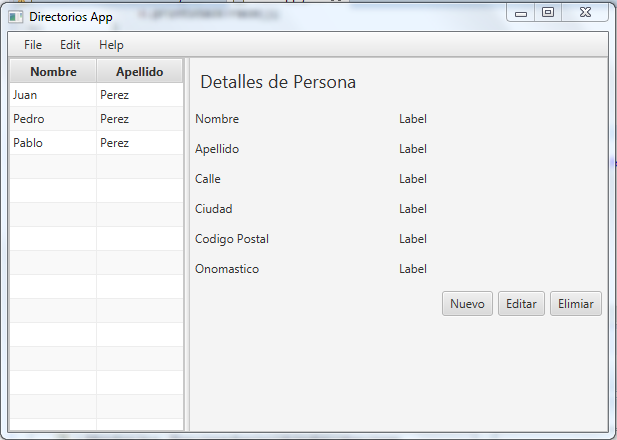
\includegraphics[width=12cm]{img/terceraParte}
\end{figure}
\section{Contenidos en Parte 2}
\begin{itemize}
	\item Creación de una clase para el modelo.
	\item Uso del modelo en una ObservableList.
	\item Visualización del modelo mediante TableView y Controladores.
\end{itemize}

\section{Crea la clase para el Modelo}
Neceistamos un modelo para contener la información sobre los contactos de nuestra agenda. Añade una nueva clase al paquete encargado de contener los modelos (\textcolor{codigo}{\texttt{ch.makery.direcciones.model}} ) denominada \textcolor{codigo}{\texttt{Persona}}. La clase \textcolor{codigo}{\texttt{Persona}} tendrá atributos (instancias de clase) para el nombre, la dirección y la fecha de nacimiento. Añade el código siguiente a la clase. Explicaré detalles de JavaFX después del código.\\
\textcolor{codigo}{\texttt{Persona.java}}
\begin{minted}[
linenos,
numbersep=5pt,
gobble=0,
frame=lines,
framesep=2mm,
breaklines=true,
]{java}

package ch.makery.direcciones.model;

import java.time.LocalDate;

import javafx.beans.property.IntegerProperty;
import javafx.beans.property.ObjectProperty;
import javafx.beans.property.SimpleIntegerProperty;
import javafx.beans.property.SimpleObjectProperty;
import javafx.beans.property.SimpleStringProperty;
import javafx.beans.property.StringProperty;

/**
* Modelo de la clase persona
* @author Mateo Mtz
*
*/
public class Persona {
	private StringProperty nombre;
	private StringProperty apellido;
	private StringProperty calle;
	private IntegerProperty codigoPostal;
	private StringProperty ciudad;
	private ObjectProperty<LocalDate> onomastico;
	public Persona(String nombre, String apellido){
		this.nombre = new SimpleStringProperty(nombre);
		this.apellido = new SimpleStringProperty(apellido);
		
		//
		this.calle = new SimpleStringProperty("Alguna calle");
		this.codigoPostal = new SimpleIntegerProperty(1234);
		this.ciudad = new SimpleStringProperty("Alguna ciudad");
		this.onomastico = new SimpleObjectProperty<LocalDate>(LocalDate.of(1999,  2,  21));
	}
	public StringProperty getNombre() {
		return nombre;
	}
	public void setNombre(String nombre) {
		this.nombre = new SimpleStringProperty(nombre);
	}
	public StringProperty getApellido() {
		return apellido;
	}
	public void setApellido(String apellido) {
		this.apellido = new SimpleStringProperty(apellido);
	}
	public StringProperty getCalle() {
		return calle;
	}
	public void setCalle(String calle) {
		this.calle = new SimpleStringProperty(calle);
	}
	public IntegerProperty getCodigoPostal() {
		return codigoPostal;
	}
	public void setCodigoPostal(int codigoPostal) {
		this.codigoPostal = new SimpleIntegerProperty(codigoPostal);
	}
	public StringProperty getCiudad() {
		return ciudad;
	}
	public void setCiudad(String ciudad) {
		this.ciudad = new SimpleStringProperty(ciudad);
	}
	public ObjectProperty<LocalDate> getOnomastico() {
		return onomastico;
	}
	public void setOnomastico(LocalDate onomastico) {
		this.onomastico = new SimpleObjectProperty<LocalDate>(onomastico);
	}
}

\end{minted}

\subsection{Explicación del código}
\begin{itemize}
	\item Con JavaFX es habitual usar \textcolor{codigo}{\texttt{Propiedades}} para todos los atributos de un clase usada como modelo. Una \textcolor{codigo}{\texttt{Propiedad}} permite, entre otras cosas, recibir notificaciones automáticamente cuando el valor de una variable cambia (por ejemplo, si cambia \textcolor{codigo}{\texttt{apellido}}. Esto ayuda a mantener sincronizados la vista y los datos. Para aprender más sobre \textcolor{codigo}{\texttt{Propiedades}} lee \textcolor{azul}{\href{https://docs.oracle.com/javase/8/javafx/properties-binding-tutorial/binding.htm}{Using JavaFX Properties and Binding}}.
	\item \textcolor{codigo}{\texttt{LocalDate}}, el tipo que usamos para especificar la fecha de nacimiento (\textcolor{codigo}{\texttt{onomastico}}) es parte de la nueva \textcolor{azul}{\href{https://docs.oracle.com/javase/tutorial/datetime/iso/}{API de JDK 8 para la fecha y la hora}}.
\end{itemize}

\section{Una lista de personas}
Los principales datos que maneja nuestra aplicación son una colección de personas. Vamos a crear una lista de objetos de tipo \textcolor{codigo}{\texttt{Persona}} dentro de la clase principal \textcolor{codigo}{\texttt{MainApp}}. El resto de controladores obtendrá luego acceso a esa lista central dentro de \textcolor{codigo}{\texttt{MainApp}}.

\subsection{Lista observable (ObservableList)}
Estas clases gráficas de JavaFX que necesitan ser informadas sobre los cambios en la lista de personas. Esto es importante, pues de otro modo la vista no estará sincronizada con los datos. Para estos fines, JavaFX ha introducido \textcolor{azul}{\href{https://docs.oracle.com/javase/8/javafx/collections-tutorial/collections.htm}{nuevas clases de colección}}.\\
De esas colecciones, necesitamos la denominada \textcolor{codigo}{\texttt{ObservableList}}. Para crear una nueva \textcolor{codigo}{\texttt{ObservableList}}, añade el código siguiente al principio de la clase \textcolor{codigo}{\texttt{MainApp}}. También añadiremos un constructor para crear datos de ejemplo y un método de consulta (get) público:\\
\textcolor{codigo}{\texttt{MainApp.java}}
\begin{minted}[
linenos,
numbersep=5pt,
gobble=0,
frame=lines,
framesep=2mm,
breaklines=true,
]{java}

	/**
	* Lista de personas en una ObservableList
	*/
	private ObservableList<Persona> personData = FXCollections.observableArrayList();
	/**
	* Constructor
	*/
	public MainApp(){
		//Agregar algunas personas a la lista
		personData.add(new Persona("Juan", "Perez"));
		personData.add(new Persona("Pedro", "Perez"));
		personData.add(new Persona("Pablo", "Perez"));
	}
	/**
	* Devuelve los datos como una lista observable de personas.
	* @return
	*/
	public ObservableList<Persona> getPersonData(){
		return personData;
	}
\end{minted}
\section{PersonOverviewController}
Finalmente vamos a añadir datos a nuestra table. Para ello necesitaremos un controlador específico para la vista \textcolor{codigo}{\texttt{PersonOverview.fxml}}.
\begin{enumerate}
	\item Crea una clase normal dentro del paquete \textbf{view} denominado \textcolor{codigo}{\texttt{PersonOverviewController.java}}. (Debemos ponerlo en el mismo paquete que \textcolor{codigo}{\texttt{PersonOverview.fxml}} o el Scene Builder no lo encontrará, al menos no en la versión actual).
	\item Añadiremos algunos atributos para acceder a la tabla y las etiquetas de la vista. Estos atributos irán precedidos por la anotación \textcolor{codigo}{\texttt{@FXML}}. Esto es necesario para que la vista tenga acceso a los atributos y métodos del controlador, incluso aunque sean privados. Una vez definida la vista en fxml, la aplicación se encargará de rellenar automáticamente estos atributos al cargar el fxml. Así pues, añade el código siguiente:
\end{enumerate}
\begin{tcolorbox}[leftrule=3mm]
	\textbf{Nota:} acuérdate siempre de importar \textbf{javafx}, NO AWT ó Swing!.
\end{tcolorbox}

\begin{minted}[
linenos,
numbersep=5pt,
gobble=0,
frame=lines,
framesep=2mm,
breaklines=true,
]{java}
package ch.makery.direcciones.view;

import ch.makery.direcciones.MainApp;
import ch.makery.direcciones.model.Persona;
import javafx.fxml.FXML;
import javafx.scene.control.Label;
import javafx.scene.control.TableColumn;
import javafx.scene.control.TableView;

public class PersonOverviewController {
	@FXML
	private TableView<Persona> personTable;
	@FXML
	private TableColumn<Persona, String> nombresColumna;
	@FXML
	private TableColumn<Persona, String> apellidosColumna;
	
	@FXML
	private Label nombreLabel;
	@FXML
	private Label apelidoLabel;
	@FXML
	private Label calleLabel;
	@FXML
	private Label codigoPostaLabel;
	@FXML
	private Label ciudadLabel;
	@FXML
	private Label onomasticoLabel;
	
	//Referencia a la clase MainApp
	private MainApp mainApp;
	/**
	* Constructor
	* Se llama al constructor antes del método initialize()
	*/
	public PersonOverviewController(){
	}
	/**
	* Inicializa la clase de controlador
	* Este método se llama automáticamente después de cargar el archivo fxml.
	*/
	@FXML
	private void initialize(){
		//Inicialice la tabla de personas con las dos columnas.
		nombresColumna.setCellValueFactory(cellData -> cellData.getValue().getNombre());
		apellidosColumna.setCellValueFactory(cellData -> cellData.getValue().getApellido());
	}
	/**
	* Es llamado por la aplicación principal para devolverse una referencia a sí mismo.
	* @param mainApp
	*/
	public void setMainApp(MainApp mainApp){
		this.mainApp = mainApp;
		personTable.setItems(mainApp.getPersonData());
	}
}

\end{minted}
Este código necesita cierta explicación:
\begin{itemize}
	\item Los campos y métodos donde el archivo fxml necesita acceso deben ser anotados con \textcolor{codigo}{\texttt{@FXML}}. En realidad, sólo si son privados, pero es mejor tenerlos privados y marcarlos con la anotación.
	\item El método \textcolor{codigo}{\texttt{initialize()}} es invocado automáticamente tras cargar el fxml. En ese momento, todos los atributos FXML deberían ya haber sido inicializados.
	\item El método \codigo{setCellValueFactory(...)} que aplicamos sobre las columnas de la tabla se usa para determinar qué atributos de la clase \codigo{Persona} deben ser usados para cada columna particular. La flecha \codigo{->} indica que estamos usando una característica de Java 8 denominada \textit{Lambdas}. Otra opción sería utilizar un \href{https://docs.oracle.com/javase/8/javafx/api/}{\codigo{\underline{PropertyValueFactory}}}, pero entonces no ofrecería seguridad de tipo (\textit{type-safe}).
\end{itemize}

\subsection{Conexión de MainApp con PersonOverviewController}
El método \codigo{setMainApp(...)} debe ser invocado desde la clase \codigo{MainApp}. Esto nos da la oportunidad de acceder al objeto \codigo{MainApp} para obtener la lista de \codigo{Persona} y otras cosas. Sustituye el método \codigo{showPersonOverview()} con el código siguiente, el cual contiene dos líneas adicionales:\\
\codigo{MainApp.java} - nuevo método \codigo{showPersonOverview()}
\begin{minted}[
linenos,
numbersep=5pt,
gobble=0,
frame=lines,
framesep=2mm,
breaklines=true,
]{java}
	/**
	* Muestra la descripción general de la persona dentro del diseño raíz.
	*/
	public void showPersonaOverview(){
		try{
			//Carga datos de persona
			FXMLLoader loader = new FXMLLoader();
			loader.setLocation(MainApp.class.getResource("view/PersonaOverview.fxml"));
			AnchorPane personaOverview = (AnchorPane) loader.load();
			
			//Carga los datos de la persona en el centro del diseño raíz.
			rootLayout.setCenter(personaOverview);
			
			//Darle al controlador acceso a la App - lineas adicionales
			PersonOverviewController controller = loader.getController();
			controller.setMainApp(this);
		}catch (IOException e) {
			e.printStackTrace();
		}
	}
\end{minted}

\section{Vincular la vista al controlador}
¡Ya casi lo tenemos! Pero falta un detalle: no le hemos indicado a la vista declarada en \codigo{PersonOverview.fxml} cuál es su controlador y que elemento hacer corresponder to cada uno de los atributos en el controlador.

\begin{enumerate}
	\item \codigo{PersonOverview.fxml} en \textit{SceneBuilder}.
	\item Abre la sección \textit{Controller} en el lado izquierdo y selecciona \codigo{PersonOverviewController} como \textbf{controlador}.
	\begin{figure}[H]
		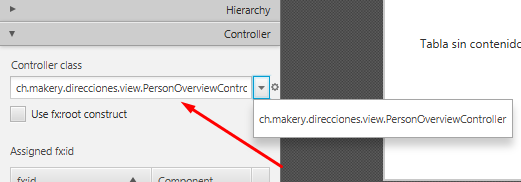
\includegraphics[width=8cm]{img/selectController}
	\end{figure}
	\item Selecciona \codigo{TableView} en la sección \textit{Hierarchy} y en el apartado \textit{Code} escribe o selecciona \codigo{personTable} en la propiedad \textbf{fx:id}.
	\begin{figure}[H]
		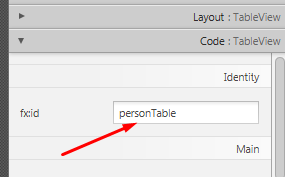
\includegraphics[width=8cm]{img/personTable}
	\end{figure}
	\item Haz lo mismo para las columnas, poniendo \codigo{nombre} y \codigo{apellido} con sus \textbf{fx:id} respectivamente.
	\item Para \textbf{cada etiqueta} en la segunda columna, introduce el \textbf{fx:id} que corresponda.
	\begin{figure}[H]
		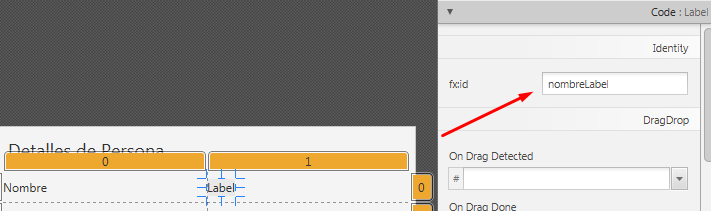
\includegraphics[width=12cm]{img/nombreLabel}
	\end{figure}
	\item Importante: En Eclipse \textbf{refresca el projecto DireccionesApp} (tecla F5). Esto es necesario porque a veces Eclipse no se da cuenta de los cambios realizados desde el \textit{Scene Builder}.
\end{enumerate}

\section{Inicia la aplicación}
Ahora, cuando ejecutes la aplicación, deberías obtener algo parecido a la captura de pantalla incluida al principio de este artículo.\\

Enhorabuena!

